\documentclass[a4paper]{article}
\usepackage{tikz}
\usepackage{geometry}
\usepackage{graphicx}
\usepackage{natbib}
\usepackage{amsmath}
\usepackage{amssymb}
\usepackage{amsthm}
\usepackage{paralist}
\usepackage{epstopdf}
\usepackage{tabularx}
\usepackage{longtable}
\usepackage{multirow}
\usepackage{multicol}
\usepackage[hidelinks]{hyperref}
\usepackage{fancyvrb}
\usepackage{algorithm}
\usepackage{algorithmic}
\usepackage{float}
\usepackage{paralist}
%\usepackage[svgname]{xcolor}
\usepackage{enumerate}
\usepackage{array}
\usepackage{times}
\usepackage{url}
\usepackage{fancyhdr}
\usepackage{comment}
\usepackage{environ}
\usepackage{times}
\usepackage{textcomp}
\usepackage{caption}
\usepackage{bbm}


\urlstyle{rm}

\setlength\parindent{0pt} % Removes all indentation from paragraphs
\theoremstyle{definition}
\newtheorem{definition}{Definition}[]
\newtheorem{conjecture}{Conjecture}[]
\newtheorem{example}{Example}[]
\newtheorem{theorem}{Theorem}[]
\newtheorem{lemma}{Lemma}
\newtheorem{proposition}{Proposition}
\newtheorem{corollary}{Corollary}

\floatname{algorithm}{Procedure}
\renewcommand{\algorithmicrequire}{\textbf{Input:}}
\renewcommand{\algorithmicensure}{\textbf{Output:}}
\newcommand{\abs}[1]{\lvert#1\rvert}
\newcommand{\norm}[1]{\lVert#1\rVert}
\newcommand{\RR}{\mathbb{R}}
\newcommand{\CC}{\mathbb{C}}
\newcommand{\Nat}{\mathbb{N}}
\newcommand{\br}[1]{\{#1\}}
\DeclareMathOperator*{\argmin}{arg\,min}
\DeclareMathOperator*{\argmax}{arg\,max}
\renewcommand{\qedsymbol}{$\blacksquare$}

\definecolor{dkgreen}{rgb}{0,0.6,0}
\definecolor{gray}{rgb}{0.5,0.5,0.5}
\definecolor{mauve}{rgb}{0.58,0,0.82}

\definecolor{C0}{HTML}{1F77B4}
\definecolor{C1}{HTML}{FF7F0E}
\definecolor{C2}{HTML}{2ca02c}
\definecolor{C3}{HTML}{d62728}
\definecolor{C4}{HTML}{9467bd}
\definecolor{C5}{HTML}{8c564b}
\definecolor{C6}{HTML}{e377c2}
\definecolor{C7}{HTML}{7F7F7F}
\definecolor{C8}{HTML}{bcbd22}
\definecolor{C9}{HTML}{17BECF}

\newcommand{\Var}{\mathrm{Var}}
\newcommand{\Cov}{\mathrm{Cov}}
\newcommand{\sgn}{\mathrm{sgn}}

\newcommand{\vc}[1]{\boldsymbol{#1}}
\newcommand{\xv}{\vc{x}}
\newcommand{\Sigmav}{\vc{\Sigma}}
\newcommand{\alphav}{\vc{\alpha}}
\newcommand{\muv}{\vc{\mu}}

\newcommand{\red}[1]{\textcolor{red}{#1}}

\def\x{\mathbf x}
\def\y{\mathbf y}
\def\w{\mathbf w}
\def\v{\mathbf v}
\def\E{\mathbb E}
\def\R{\mathbb R}
\def\V{\mathbb V}
\def\ind{\mathbbm 1}

% TO SHOW SOLUTIONS, include following (else comment out):
\newenvironment{soln}{
    \leavevmode\color{blue}\ignorespaces
}{}


\hypersetup{
%    colorlinks,
    linkcolor={red!50!black},
    citecolor={blue!50!black},
    urlcolor={blue!80!black}
}

\geometry{
  top=1in,            % <-- you want to adjust this
  inner=1in,
  outer=1in,
  bottom=1in,
  headheight=3em,       % <-- and this
  headsep=2em,          % <-- and this
  footskip=3em,
}


\pagestyle{fancyplain}
\lhead{\fancyplain{}{Homework 8}}
\rhead{\fancyplain{}{CS 760 Machine Learning}}
\cfoot{\thepage}

\title{\textsc{Homework 8}} % Title

%%% NOTE:  Replace 'NAME HERE' etc., and delete any "\red{}" wrappers (so it won't show up as red)

\author{
\red{$>>$NAME HERE$<<$} \\
\red{$>>$ID HERE$<<$}\\
} 

\date{}

\begin{document}

\maketitle 


\textbf{Instructions:} 
Although this is a programming homework, you only need to hand in a pdf answer file.
There is no need to submit the latex source or any code.
You can choose any programming language, as long as you implement the algorithm from scratch.

Use this latex file as a template to develop your homework.
Submit your homework on time as a single pdf file to Canvas.
Please check Piazza for updates about the homework.


\section{Principal Component Analysis [50 pts]}
Download three.txt and eight.txt.  Each has 200 handwritten digits.  Each line is for a digit, vectorized from a 16x16 gray scale image.  
\begin{enumerate}
\item (5 pts) Each line has 256 numbers: they are pixel values (0=black, 255=white) vectorized from the image as the first column (top down), the second column, and so on.
Visualize the two gray scale images corresponding to the first line in three.txt and the first line in eight.txt.

\item (5 pts) Putting the two data files together (threes first, eights next) to form a $n \times D$ matrix $X$ where $n=400$ digits and $D=256$ pixels.  Note we use $n\times D$ size for $X$ instead of $D\times n$ to be consistent with the convention in linear regression.   The $i$th row of $X$ is $x_i^\top$, where $x_i \in \R^D$ is the $i$th image in the combined data set.
Compute the sample mean $y = {1\over n} \sum_{i=1}^n x_i$.
Visualize $y$ as a 16x16 gray scale image.

\item (10 pts) Center $X$ using $y$ above.  Then form the sample covariance matrix $S={X^\top X \over n-1}$.
Show the 5x5 submatrix $S(1\ldots 5, 1 \ldots 5)$.

\item (10 pts) Use appropriate software to compute the two largest eigenvalues $\lambda_1 \ge \lambda_2$ and the corresponding eigenvectors $v_1, v_2$ of $S$.
For example, in Matlab one can use eigs(S,2).  
Show the value of $\lambda_1, \lambda_2$.
Visualize $v_1, v_2$ as two 16x16 gray scale images.
Hint: their elements will not be in [0, 255], but you can shift and scale them appropriately.  It is best if you can show an accompany ``colorbar'' that maps gray scale to values. 

\item (5 pts) Now we project (the centered) $X$ down to the two PCA directions.   Let $V=[v_1 v_2]$ be the $D\times 2$ matrix.  The projection is simply $XV$.
Show the resulting two coordinates for the first line in three.txt and the first line in eight.txt, respectively.

\item (5 pts) Now plot the 2D point cloud of the 400 digits after projection.
For visual interest, color points in three.txt red and points in eight.txt blue.
But keep in mind that PCA is an unsupervised learning method and it does not know such class labels.

\end{enumerate}




\section{Q-learning [50 pts]}
Consider the following Markov Decision Process.
It has two states $s$.
It has two actions $a$: move and stay.
The state transition is deterministic: ``move'' moves to the other state, while ``stay' stays at the current state.
The reward $r$ is 0 for move,  1 for stay. 
There is a discounting factor $\gamma=0.9$.
\\
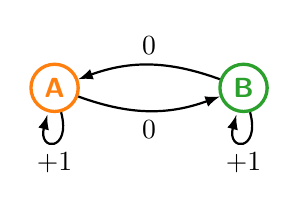
\begin{tikzpicture}
\tikzstyle{n} = [very thick,circle,inner sep=0mm,minimum width=6mm]
\tikzstyle{a} = [thick,>=latex,->]
\def\dx{1.2}
\def\dy{-1.2}
\node[n,C1,draw=C1] (2) at (\dy,0) {\textbf{\textsf{A}}};
\node[n,C2,draw=C2] (1) at (\dx,0) {\textbf{\textsf{B}}};
\path[a]
(2) edge [loop below] node {+1}(2)
(1) edge [loop below] node {+1}(1)
(2) edge [bend right=20] node[below] {0}(1)
(1) edge [bend right=20] node[above] {0}(2);
\end{tikzpicture}

The reinforcement learning agent performs Q-learning.  Recall the $Q$ table has entries $Q(s,a)$.
The $Q$ table is initialized with all zeros.
The agent starts in state $s_1=A$.
In any state $s_t$, the agent chooses the action $a_t$ according to a behavior policy $a_t = \pi_B(s_t)$.
Upon experiencing the next state and reward $s_{t+1}, r_t$ the update is:
$$Q(s_t, a_t) \Leftarrow (1-\alpha) Q(s_t, a_t) + \alpha \left( r_t + \gamma \max_{a'} Q(s_{t+1}, a') \right).$$
Let the step size parameter $\alpha=0.5$.

\begin{enumerate}
\item Run Q-learning for 200 steps with a uniformly random behavior policy: $\pi_B(s_t)=$ move or stay with 1/2 probability for any $s_t$.
Show the Q table at the end.



\item Reset and repeat the above, but with an $\epsilon$-greedy behavior policy: at each state $s_t$, with probability $1-\epsilon$ choose what the current Q table says is the best action: $\argmax_a Q(s_t,a)$; Break ties arbitrarily. Otherwise (with probability $\epsilon$) uniformly chooses between move and stay.
Use $\epsilon=0.5$.


\item Reset and repeat the above, but with a deterministic greedy behavior policy: at each state $s_t$ use the best action $a_t \in \argmax_a Q(s_t,a)$ indicated by the current Q table. If there is a tie, prefer move.

\item Without doing simulation, use Bellman equation to derive the true Q table induced by the MDP.

\end{enumerate}


\section{Extra Credit: VC dimension [10 pts]}
Let the input $x\in X=\R$.
Consider $F=\{f(x)=\sgn(ax^2+bx+c): a, b, c \in \R\}$, where $\sgn(z)=1$ if $z\ge0$, and 0 otherwise.
What is $VC(F)$?  Prove it.



\section{Extra Credit: VC-dimension of Linear Separators [10 pts]}
In this problem, you will prove that the VC-dimension of the class $H_n$ of halfspaces (another term for linear threshold functions $f_{w,b}(x) = \text{sign}(w^\top x + b)$) in $n$ dimensions is $n+1$. We will use the following definition: The convex hull of a set of points $S$ is the set of all convex combinations of points in $S$; this is the set of all points that can be written as $\sum_{x_i \in S} \lambda_i x_i$, where each $\lambda_i \ge 0$, and $\sum_i \lambda_i = 1$. It is not hard to see that if a halfspace has all points from a set $S$ on one side, then the entire convex hull of $S$ must be on that side as well. 

(a) [lower bound] Prove that $\text{VC-dim}(H_n) \ge n+1$ by presenting a set of $n+1$ points in $n$-dimension space such that one can partition that set with halfspaces in all possible ways, i.e., the set of points are shattered by $H_n$. (And, show how one can partition the set in any desired way.)

(b) [upper bound part 1] The following is Radon's Theorem, from 1920's. 
\begin{theorem} 
Let $S$ be a set of $n+2$ points in $n$ dimensions. Then $S$ can be partitioned into two (disjoint) subsets $S_1$ and $S_2$ whose convex hulls intersect. 
\end{theorem}
Show that Radon's Theorem implies that the VC-dimension of halfspaces is at most $n+1$. Conclude that $\text{VC-dim}(H_n) = n+1$.

(c) [upper bound part 2] Now we prove Radon's Theorem. We will need the following standard fact from linear algebra. If $x_1, \ldots, x_{n+1}$ are $n+1$ points in $n$-dimensional space, then they are linearly dependent. That is, there exist real values $\lambda_1, \ldots, \lambda_{n+1}$ not all zero such that $\lambda_1 x_1 + \ldots + \lambda_{n+1} x_{n+1} = 0$.
You may now prove Radon's Theorem however you wish. However, as a suggested first step, prove the following. For any set of $n+2$ points $x_1, \ldots, x_{n+2}$ in $n$-dimensional space, there exist $\lambda_1, \ldots, \lambda_{n+2}$ not all zero such that $\sum_i \lambda_i x_i = 0$ and $\sum_i \lambda_i = 0$. (This is called affine dependence.)


\end{document}
